\documentclass[]{article}
\usepackage{listings}
\usepackage[MeX]{polski}
\usepackage[utf8]{inputenc}
\usepackage{graphicx}
\usepackage{xcolor}
\usepackage{float}
\usepackage{ulem}
\usepackage{placeins}
\usepackage{listings}
\definecolor{verilogcommentcolor}{RGB}{104,180,104}
\definecolor{verilogkeywordcolor}{RGB}{49,49,255}
\definecolor{verilogsystemcolor}{RGB}{128,0,255}
\definecolor{verilognumbercolor}{RGB}{255,143,102}
\definecolor{verilogstringcolor}{RGB}{160,160,160}
\definecolor{verilogdefinecolor}{RGB}{128,64,0}
\definecolor{verilogoperatorcolor}{RGB}{0,0,128}

% Verilog style
\lstdefinestyle{prettyverilog}{
   language           = Verilog,
   commentstyle       = \color{verilogcommentcolor},
   alsoletter         = \$'0123456789\`,
   literate           = *{+}{{\verilogColorOperator{+}}}{1}%
                         {-}{{\verilogColorOperator{-}}}{1}%
                         {@}{{\verilogColorOperator{@}}}{1}%
                         {;}{{\verilogColorOperator{;}}}{1}%
                         {*}{{\verilogColorOperator{*}}}{1}%
                         {?}{{\verilogColorOperator{?}}}{1}%
                         {:}{{\verilogColorOperator{:}}}{1}%
                         {<}{{\verilogColorOperator{<}}}{1}%
                         {>}{{\verilogColorOperator{>}}}{1}%
                         {=}{{\verilogColorOperator{=}}}{1}%
                         {!}{{\verilogColorOperator{!}}}{1}%
                         {^}{{\verilogColorOperator{^}}}{1}%
                         {|}{{\verilogColorOperator{|}}}{1}%
                         {=}{{\verilogColorOperator{=}}}{1}%
                         {[}{{\verilogColorOperator{[}}}{1}%
                         {]}{{\verilogColorOperator{]}}}{1}%
                         {(}{{\verilogColorOperator{(}}}{1}%
                         {)}{{\verilogColorOperator{)}}}{1}%
                         {,}{{\verilogColorOperator{,}}}{1}%
                         {.}{{\verilogColorOperator{.}}}{1}%
                         {~}{{\verilogColorOperator{$\sim$}}}{1}%
                         {\%}{{\verilogColorOperator{\%}}}{1}%
                         {\&}{{\verilogColorOperator{\&}}}{1}%
                         {\#}{{\verilogColorOperator{\#}}}{1}%
                         {\ /\ }{{\verilogColorOperator{\ /\ }}}{3}%
                         {\ _}{\ \_}{2}%
                        ,
   morestring         = [s][\color{verilogstringcolor}]{"}{"},%
   identifierstyle    = \color{black},
   vlogdefinestyle    = \color{verilogdefinecolor},
   vlogconstantstyle  = \color{verilognumbercolor},
   vlogsystemstyle    = \color{verilogsystemcolor},
   basicstyle         = \scriptsize\fontencoding{T1}\ttfamily,
   keywordstyle       = \bfseries\color{verilogkeywordcolor},
   numbers            = left,
   numbersep          = 10pt,
   tabsize            = 4,
   escapeinside       = {/*!}{!*/},
   upquote            = true,
   sensitive          = true,
   showstringspaces   = false, %without this there will be a symbol in the places where there is a space
   frame              = single
}


% This is shamelessly stolen and modified from:
% https://github.com/jubobs/sclang-prettifier/blob/master/sclang-prettifier.dtx
\makeatletter

% Language name
\newcommand\language@verilog{Verilog}
\expandafter\lst@NormedDef\expandafter\languageNormedDefd@verilog%
  \expandafter{\language@verilog}
  
% save definition of single quote for testing
\lst@SaveOutputDef{`'}\quotesngl@verilog
\lst@SaveOutputDef{``}\backtick@verilog
\lst@SaveOutputDef{`\$}\dollar@verilog

% Extract first character token in sequence and store in macro 
% firstchar@verilog, per http://tex.stackexchange.com/a/159267/21891
\newcommand\getfirstchar@verilog{}
\newcommand\getfirstchar@@verilog{}
\newcommand\firstchar@verilog{}
\def\getfirstchar@verilog#1{\getfirstchar@@verilog#1\relax}
\def\getfirstchar@@verilog#1#2\relax{\def\firstchar@verilog{#1}}

% Initially empty hook for lst
\newcommand\addedToOutput@verilog{}
\lst@AddToHook{Output}{\addedToOutput@verilog}

% The style used for constants as set in lstdefinestyle
\newcommand\constantstyle@verilog{}
\lst@Key{vlogconstantstyle}\relax%
   {\def\constantstyle@verilog{#1}}

% The style used for defines as set in lstdefinestyle
\newcommand\definestyle@verilog{}
\lst@Key{vlogdefinestyle}\relax%
   {\def\definestyle@verilog{#1}}

% The style used for defines as set in lstdefinestyle
\newcommand\systemstyle@verilog{}
\lst@Key{vlogsystemstyle}\relax%
   {\def\systemstyle@verilog{#1}}

% Counter used to check current character is a digit
\newcount\currentchar@verilog
  
% Processing macro
\newcommand\@ddedToOutput@verilog
{%
   % If we're in \lstpkg{}' processing mode...
   \ifnum\lst@mode=\lst@Pmode%
      % Save the first token in the current identifier to \@getfirstchar
      \expandafter\getfirstchar@verilog\expandafter{\the\lst@token}%
      % Check if the token is a backtick
      \expandafter\ifx\firstchar@verilog\backtick@verilog
         % If so, then this starts a define
         \let\lst@thestyle\definestyle@verilog%
      \else
         % Check if the token is a dollar
         \expandafter\ifx\firstchar@verilog\dollar@verilog
            % If so, then this starts a system command
            \let\lst@thestyle\systemstyle@verilog%
         \else
            % Check if the token starts with a single quote
            \expandafter\ifx\firstchar@verilog\quotesngl@verilog
               % If so, then this starts a constant without length
               \let\lst@thestyle\constantstyle@verilog%
            \else
               \currentchar@verilog=48
               \loop
                  \expandafter\ifnum%
                  \expandafter`\firstchar@verilog=\currentchar@verilog%
                     \let\lst@thestyle\constantstyle@verilog%
                     \let\iterate\relax%
                  \fi
                  \advance\currentchar@verilog by \@ne%
                  \unless\ifnum\currentchar@verilog>57%
               \repeat%
            \fi
         \fi
      \fi
      % ...but override by keyword style if a keyword is detected!
      %\lsthk@DetectKeywords% 
   \fi
}

% Add processing macro only if verilog
\lst@AddToHook{PreInit}{%
  \ifx\lst@language\languageNormedDefd@verilog%
    \let\addedToOutput@verilog\@ddedToOutput@verilog%
  \fi
}

% Colour operators in literate
\newcommand{\verilogColorOperator}[1]
{%
  \ifnum\lst@mode=\lst@Pmode\relax%
   {\bfseries\textcolor{verilogoperatorcolor}{#1}}%
  \else
    #1%
  \fi
}

\makeatother

\usepackage{trace}
\title{TECY - Projekt 2}
\author{Małgorzata Pszczółkowska - 311423\\ Anastasiya Ronskaya - 317058 \\ Konrad Kotlicki - 310958 \\Sebastian Skrzek - 311442}
\begin{document}
\maketitle
\tableofcontents
\section{Funkcja}
Funkcja F(x5,x4,x3,x2,x1,x0) podana jest w postaci tabeli:
\newline
\newline
\begin{tabular}[]{|c|c|}
\hline
   \footnotesize{x5x4x3x2x1x0} & \footnotesize{y1y0}\\
\hline   
   100100 & 00\\
   101110 & 01\\
   110111 & 01\\
   101100 & 00\\
   001110 & 10\\
   110100 & 10\\
   100111 & 10\\
   001011 & 11\\
   001010 & 11\\
\hline
\end{tabular}
\section{Dekompozycja 1}
 Istnieje dekompozycja F = H(x2,x1,x0), G(x5,x4,x3)
\newline
 Dekompozycja jest dla G=(x5,x4,x3) i funkcja G ma postać:
\newline
\newline
\begin{tabular}[]{|c|c|}
\hline
   \footnotesize{x5x4x3} & \footnotesize{g}\\
\hline   
   000 & -\\
   001 & 1\\
   010 & -\\
   011 & -\\
   100 & 0\\
   101 & 0\\
   110 & 1\\
   111 & -\\
\hline
\end{tabular}
\newline
\newline
Funkcja H ma postać H =(x2,x1,x0,g):
\newline
\newline
\begin{tabular}[]{|c|c|c|}
\hline
   \footnotesize{x2x1x0/g} & \footnotesize{0} & \footnotesize{1}\\
\hline   
   000 & -- & --\\
   001 & -- & --\\
   010 & -- & 11\\
   011 & -- & 11\\
   100 & 00 & 10\\
   101 & -- & --\\
   110 & 01 & 10\\
   111 & 10 & 01\\
\hline
\end{tabular}
\newline
\newline
\begin{figure}[H]
	\centering
	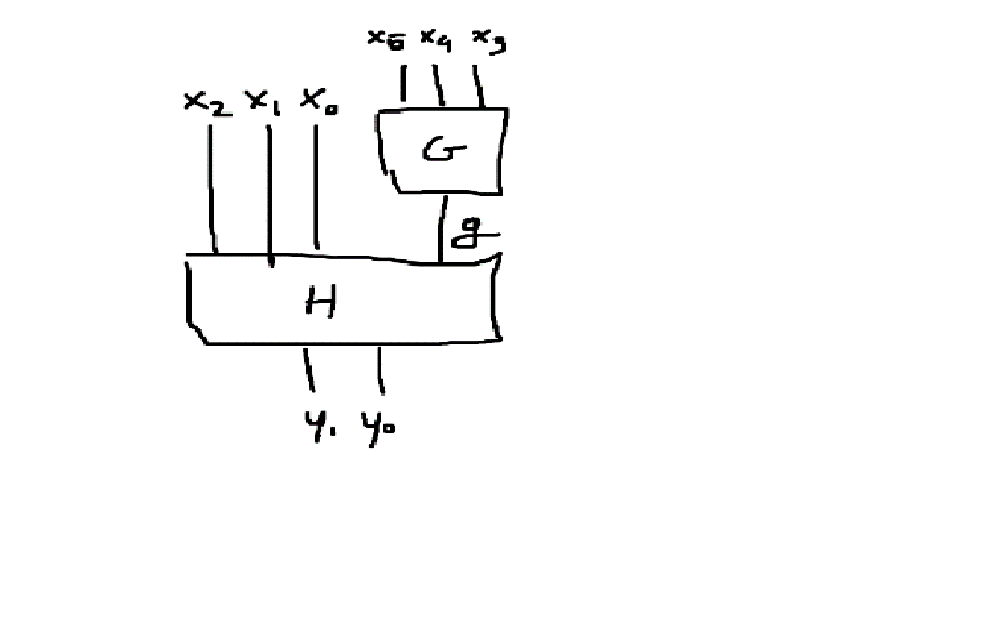
\includegraphics[width=0.65\textwidth]{1.0.png}
\end{figure}
\newpage
\subsection{Realizacja w Logisim}
Funkcja F ma 6 bitów wejściowych i 2 wyjściowe
\begin{figure}[H]
	\centering
	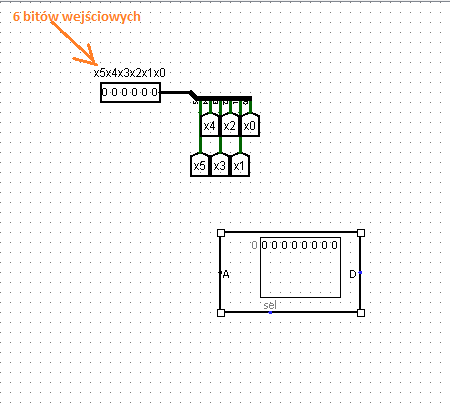
\includegraphics[width=0.65\textwidth]{1.1.png}
\end{figure}
Funkcja G ma 3 bity wejściowe i 1 bit wyjściowy
\begin{figure}[H]
	\centering
	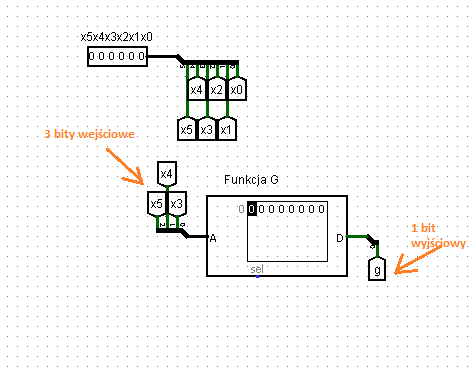
\includegraphics[width=0.65\textwidth]{1.2.png}
\end{figure}
\newpage
Zawartość pamięci ROM dla funkcji G
\begin{figure}[H]
	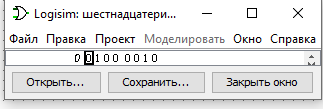
\includegraphics[width=0.65\textwidth]{1.3.png}
\end{figure}
Funkcja H ma 4 bity wejściowe i 2 wyjściowe
\begin{figure}[H]
	\centering
	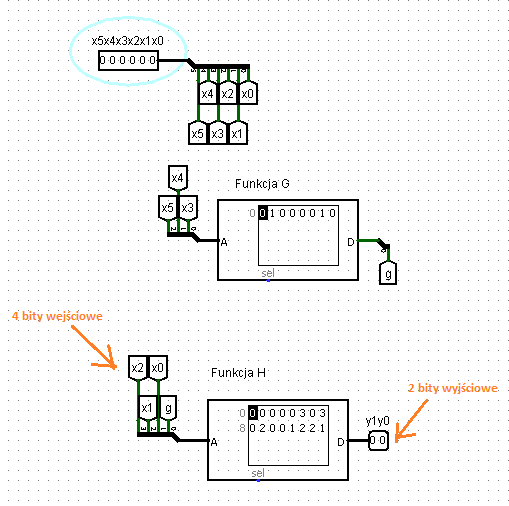
\includegraphics[width=0.65\textwidth]{1.4.png}
\end{figure}
Zawartość pamięci ROM dla funkcji H
\begin{figure}[H]
	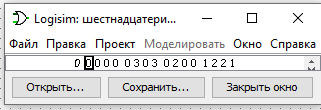
\includegraphics[width=0.65\textwidth]{1.5.png}
\end{figure}
\newpage
\begin{center}
    TESTY
\end{center}
x5x4x3x2x1x1=100100
\begin{figure}[H]
	\centering
	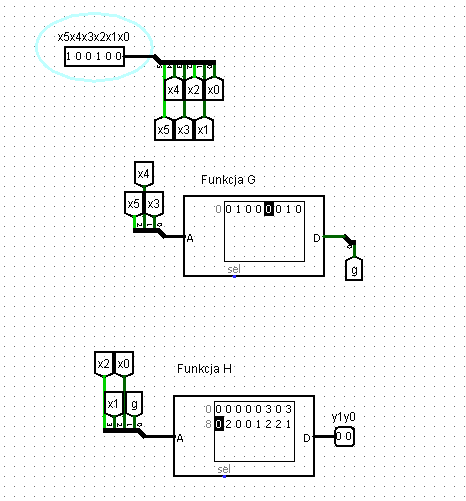
\includegraphics[width=0.60\textwidth]{1.6.png}
\end{figure}
x5x4x3x2x1x1=101110
\begin{figure}[H]
	\centering
	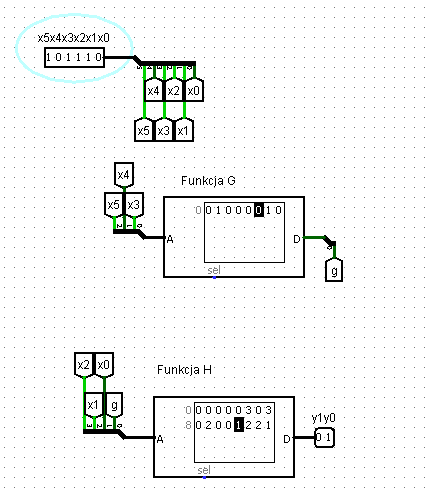
\includegraphics[width=0.60\textwidth]{1.7.png}
\end{figure}
x5x4x3x2x1x1=110111
\begin{figure}[H]
	\centering
	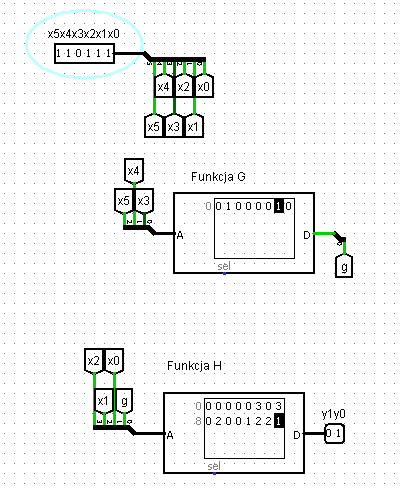
\includegraphics[width=0.57\textwidth]{1.8.png}
\end{figure}
x5x4x3x2x1x1=101100
\begin{figure}[H]
	\centering
	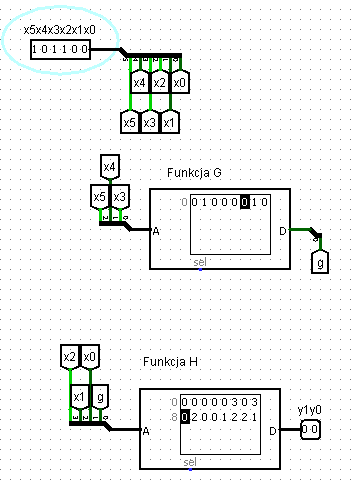
\includegraphics[width=0.50\textwidth]{1.9.png}
\end{figure}
\newpage
x5x4x3x2x1x1=001110
\begin{figure}[H]
	\centering
	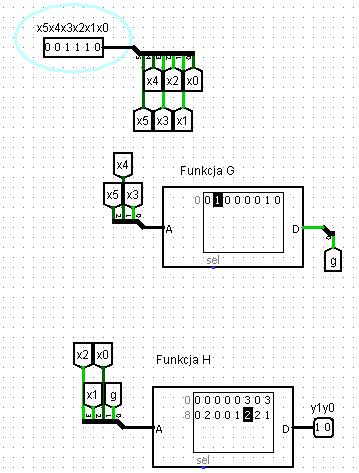
\includegraphics[width=0.53\textwidth]{1.10.png}
\end{figure}
x5x4x3x2x1x1=110100
\begin{figure}[H]
	\centering
	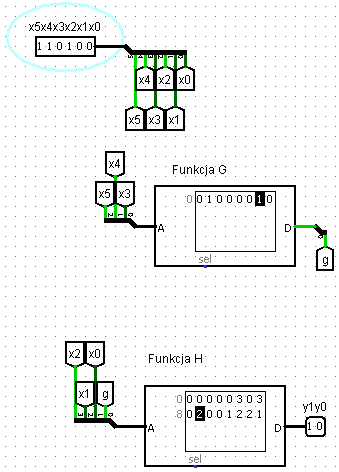
\includegraphics[width=0.53\textwidth]{1.11.png}
\end{figure}
x5x4x3x2x1x1=100111
\begin{figure}[H]
	\centering
	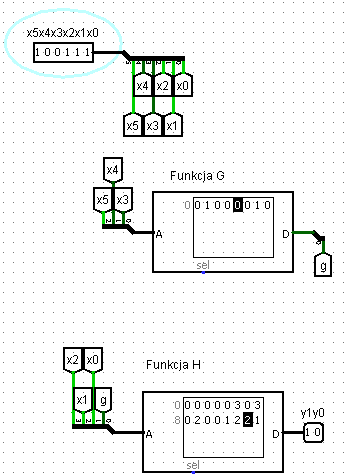
\includegraphics[width=0.53\textwidth]{1.12.png}
\end{figure}
x5x4x3x2x1x1=001011
\begin{figure}[H]
	\centering
	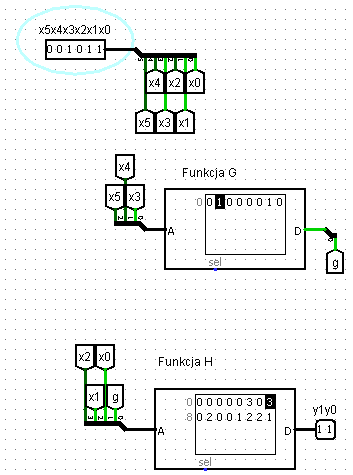
\includegraphics[width=0.52\textwidth]{1.13.png}
\end{figure}
x5x4x3x2x1x1=001010
\begin{figure}[H]
	\centering
	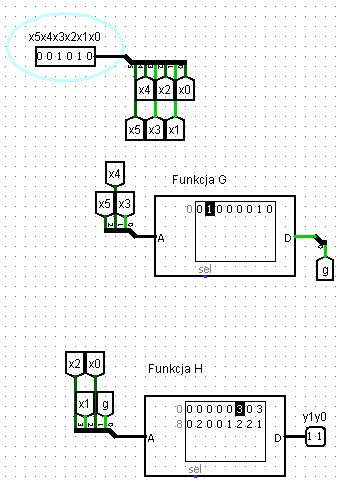
\includegraphics[width=0.55\textwidth]{1.14.png}
\end{figure}
\subsection{Realizacja w Quartus}
Tworzymy plik Verilog HDL File o nazwie funkcja\_f. Zakodujemy funkcję F. 
\newline
Zawartość pliku funkcja\_f:
\begin{lstlisting}[style={prettyverilog}]
module funkcja_f
(   
    input x5,x4,x3,x2,x1,x0,
	 output y1,y0
);	 
wire g;
 
funkcja_g b0 (.x5(x5),.x4(x4),.x3(x3),.g(g));
funkcja_h b1 (.x2(x2),.x1(x1),.x0(x0),.g(g),.y1(y1),.y0(y0));
 
endmodule
\end{lstlisting}
\begin{figure}[H]
	\centering
	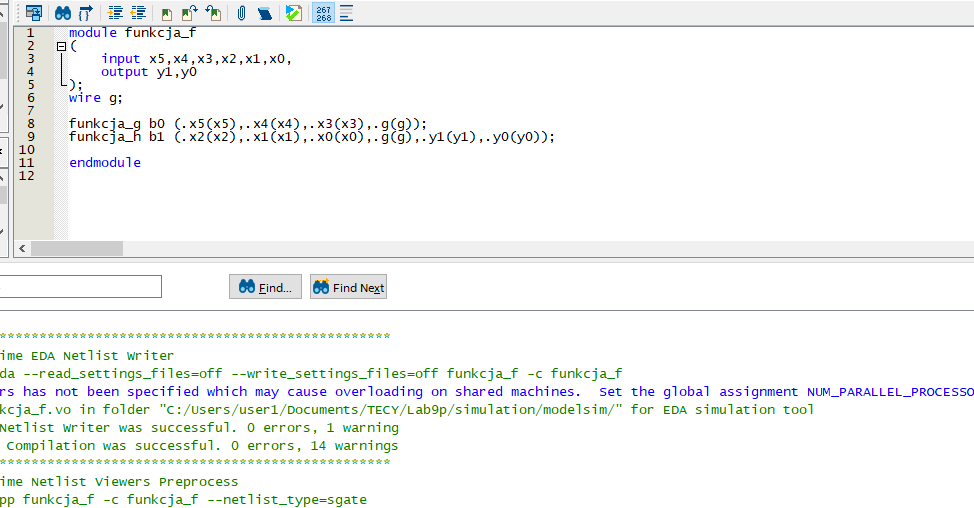
\includegraphics[width=1.39\textwidth]{1.15.png}
\end{figure}

Tworzymy nowy plik Verilog HDL File o nazwie funkcja\_g. Zakodujemy funkcję G. 
\newline
Zawartość pliku funkcja\_g:
\begin{lstlisting}[style={prettyverilog}]
module funkcja_g
(
    input x5, x4, x3,
	 output g

);
reg temp;

always@* 
	case ({x5,x4,x3}) 
		3'd4 : temp = 1'd0;
		3'd5 : temp = 1'd0;
		3'd6 : temp = 1'd1;
		3'd1 : temp = 1'd1;
	   default: temp = 1'd0;
    endcase
assign {g} = temp;	 
endmodule

\end{lstlisting}
\begin{figure}[H]
	\centering
	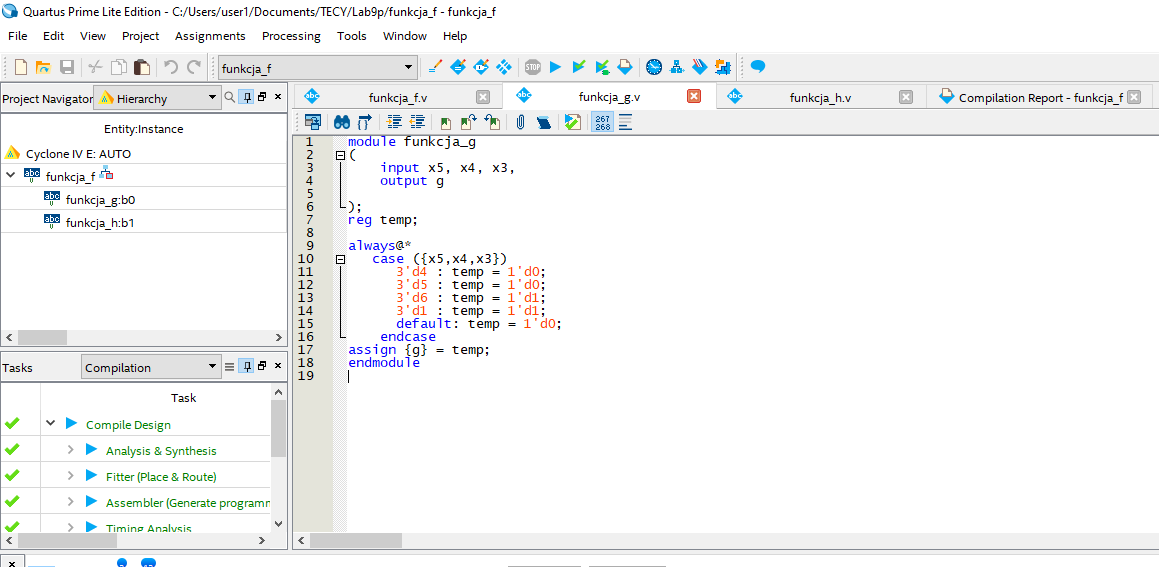
\includegraphics[width=1.39\textwidth]{1.16.png}
\end{figure}
Tworzymy nowy plik Verilog HDL File o nazwie funkcja\_h. Zakodujemy funkcję H. 
\newline
Zawartość pliku funkcja\_h:
\begin{lstlisting}[style={prettyverilog}]
module funkcja_h
(
    input x2, x1, x0, g,
	 output y1,y0

);
reg [0:1] temp;
always@* 
	case ({x2,x1,x0,g}) 
		//4'd0 : temp = 2'd0;
		//4'd1 : temp = 2'd0;
		//4'd2 : temp = 2'd1;
		//4'd3 : temp = 2'd1;
		
		//4'd4 : temp = 2'd0;
		4'd5 : temp = 2'd3;
		//4'd6 : temp = 2'd0;
		4'd7 : temp = 2'd3;
		
		4'd8 : temp = 2'd0;
		4'd9 : temp = 2'd2;
		//4'd10 : temp = 2'd0;
		//4'd11 : temp = 2'd0;
		
		4'd12 : temp = 2'd1;
		4'd13 : temp = 2'd2;
		4'd14 : temp = 2'd2;
		4'd15 : temp = 2'd1;
	   default: temp = 2'd0;
    endcase
assign {y1,y0} = temp;	 
endmodule
\end{lstlisting}
\begin{figure}[H]
	\centering
	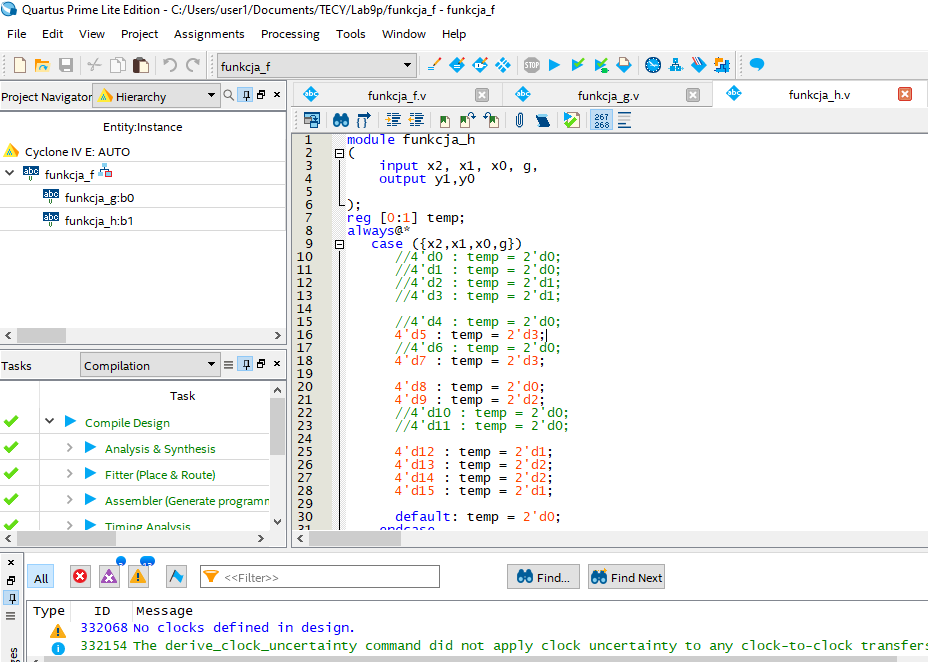
\includegraphics[width=1.39\textwidth]{1.17.png}
\end{figure}
\begin{center}
    STRUKTURA
\end{center}
\begin{figure}[H]
	\centering
	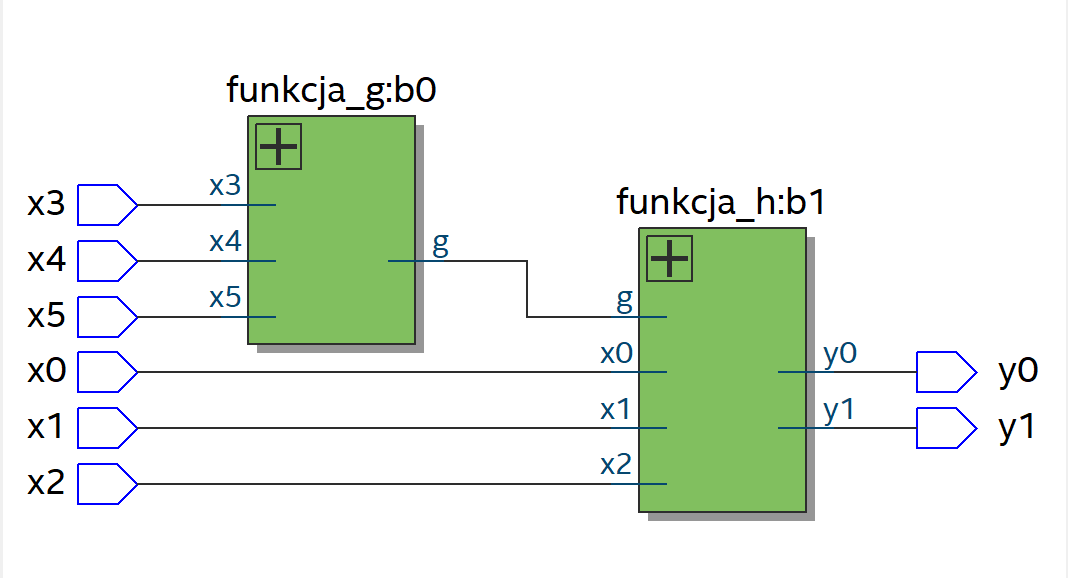
\includegraphics[width=0.70\textwidth]{1.18.png}
\end{figure}
\begin{center}
    Compilation Report
\end{center}
\begin{figure}[H]{l}
	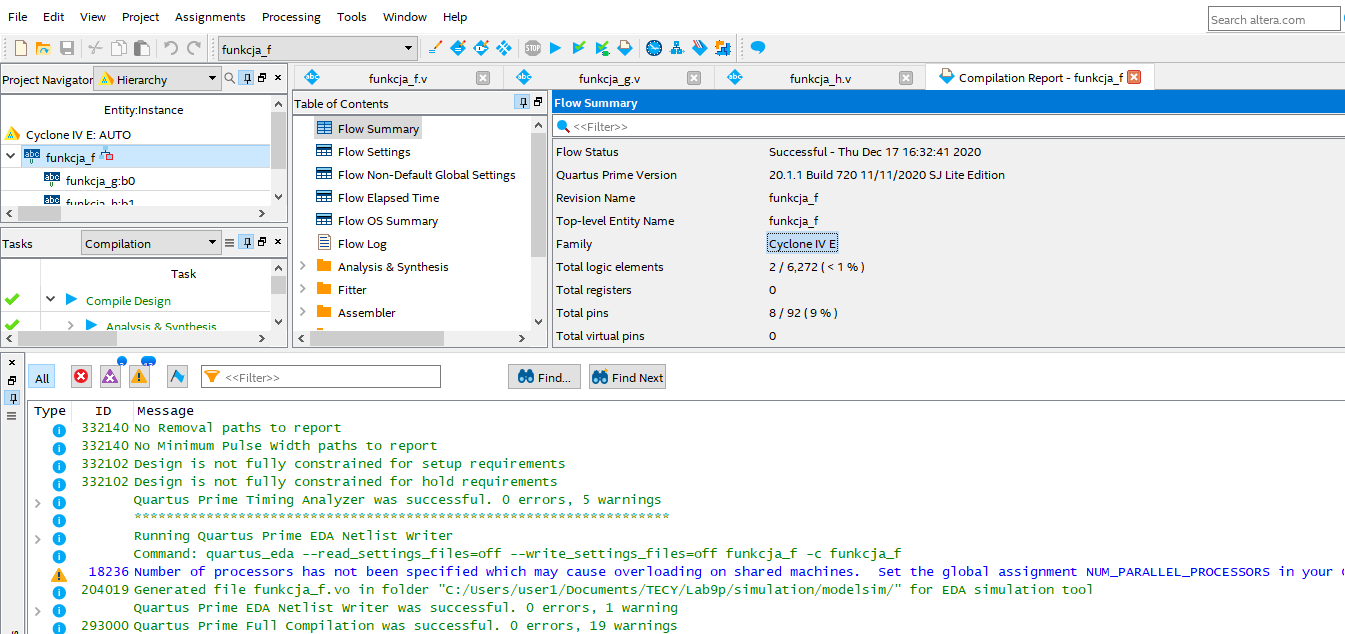
\includegraphics[width=1.50\textwidth]{1.19.png}
\end{figure}
\newpage
\subsection{Weryfikacja w ModelSim}
\par Przeprowadzamy symulację w ModelSim.
\begin{figure}[H]
	\centering
	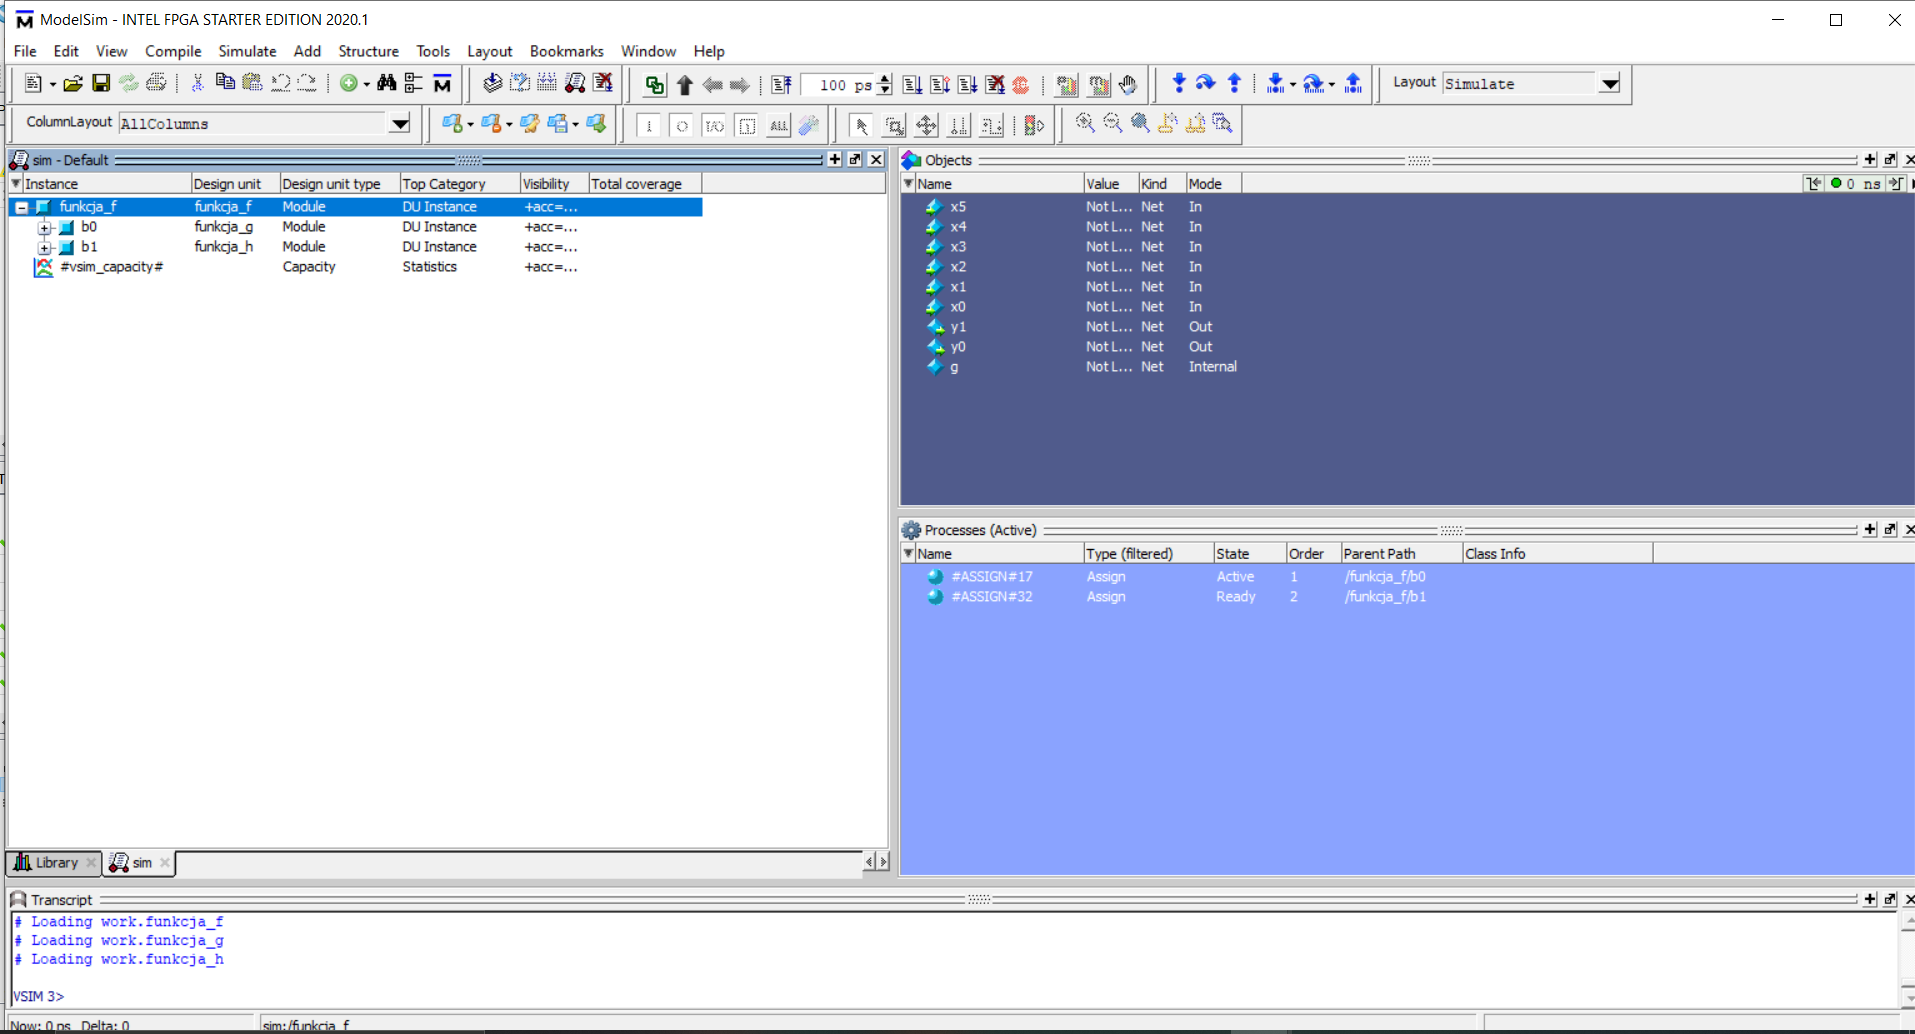
\includegraphics[width=1.25\textwidth]{modelsim1.png}
	\caption{Widok okna ModelSim}
\end{figure}
Sprawdzamy poprawność wyników dla wejść podanych w tabeli prawdy funkcji F. 
\newpage
Zawartość pliku testującego test\_f.do:

\begin{minipage}{0.5\textwidth}
\begin{figure}[H]
	\centering
	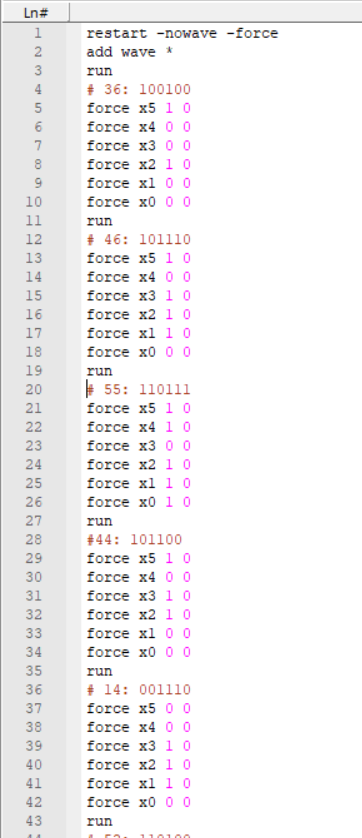
\includegraphics[width=1\textwidth]{test_f1_1.png}
\end{figure}
\end{minipage}
\begin{minipage}{0.5\textwidth}
\begin{figure}[H]
	\centering
	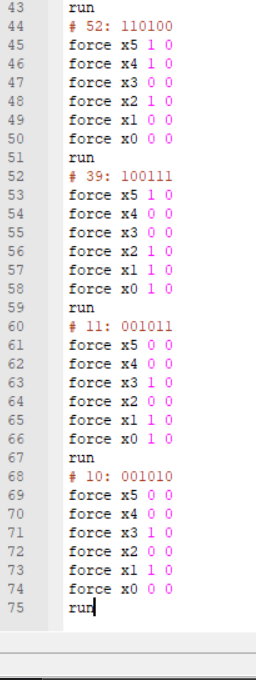
\includegraphics[width=1\textwidth]{test_f1_2.png}
\end{figure}
\end{minipage}
\newpage
\par Widok okna Wave po wykonaniu przez ModelSim polecenia $>$do test\_f.do:
\begin{figure}[H]
	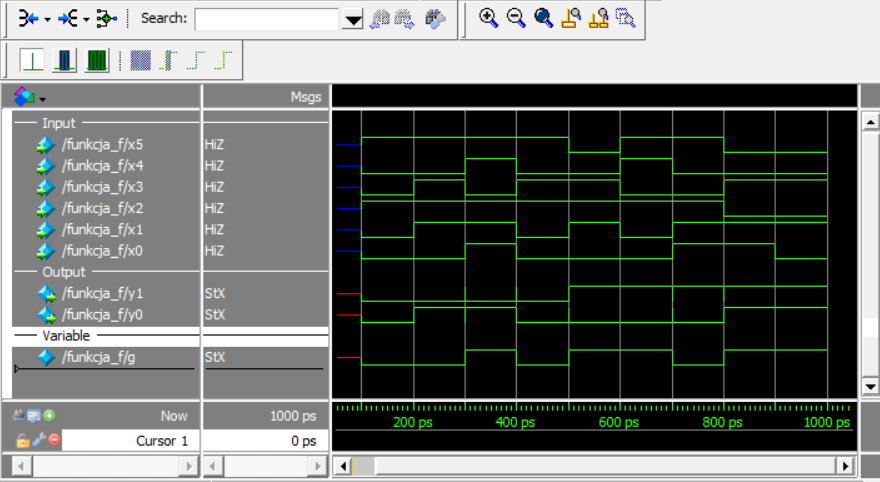
\includegraphics[width=1.25\textwidth]{wave.png}
\end{figure}
Na podstawie otrzymanych sygnałów zapiszemy tabelę:
\\
\\
\begin{tabular}[]{|c c c c c c |c c|}
\hline
$x_5$ & $x_4$ & $x_3$ & $x_2$ & $x_1$ & $x_0$ & $y_1$ & $y_0$ \\\hline
1 & 0 & 0 & 1 & 0 & 0 & 0 & 0\\
1 & 0 & 1 & 1 & 1 & 0 & 0 & 1\\
1 & 1 & 0 & 1 & 1 & 1 & 0 & 1\\
1 & 0 & 1 & 1 & 0 & 0 & 0 & 0\\
0 & 0 & 1 & 1 & 0 & 0 & 1 & 0\\
1 & 1 & 0 & 1 & 0 & 0 & 1 & 0\\
1 & 0 & 0 & 1 & 1 & 1 & 1 & 0\\
0 & 0 & 1 & 0 & 1 & 1 & 1 & 1\\
0 & 0 & 1 & 0 & 1 & 0 & 1 & 1\\ \hline
\end{tabular}
\\
\\ \textbf{Powstała tabela zgadza się z podaną w treści zadania tabelą funkcji F.}
\section{Dekompozycja 3}
 Istneje też dekompozycja F= H(G1(x4,x2,x1), G(x5,x4,x3), x0)
\newline
funkcja G ma postać:
\newline
\newline
\begin{tabular}[]{|c|c|}
\hline
   \footnotesize{x5x4x3} & \footnotesize{g}\\
\hline   
   000 & -\\
   001 & 1\\
   010 & -\\
   011 & -\\
   100 & 0\\
   101 & 0\\
   110 & 1\\
   111 & -\\
\hline
\end{tabular}
\newline
\newline
Funkcja G1 ma postać:
\newline
\newline
\begin{tabular}[]{|c|c|}
\hline
   \footnotesize{x4x2x1} & \footnotesize{g2}\\
\hline   
   000 & -\\
   001 & 0\\
   010 & 0\\
   011 & 1\\
   100 & -\\
   101 & -\\
   110 & 1\\
   111 & 1\\
\hline
\end{tabular}
\newline
\newline
Funkcja H ma postać:
\newline
\newline
\begin{tabular}[]{|c|c|c|}
\hline
   \footnotesize{x0 g/g2} & \footnotesize{0} & \footnotesize{1}\\
\hline   
   00 & 00 & 01\\
   01 & 11 & 10\\
   10 & 11 & 10\\
   11 & 11 & 01\\
\hline
\end{tabular}
\begin{figure}[H]
	\centering
	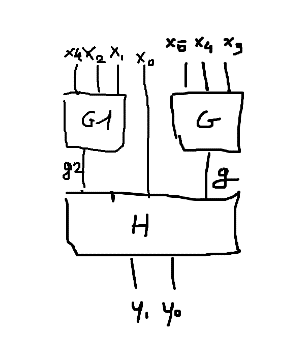
\includegraphics[width=0.50\textwidth]{schemat3.png}
\end{figure}
\subsection{Realizacja w Logisim}
Funkcja F ma 6 bitów wejściowych i 2 wyjściowe
\begin{figure}[H]
	\centering
	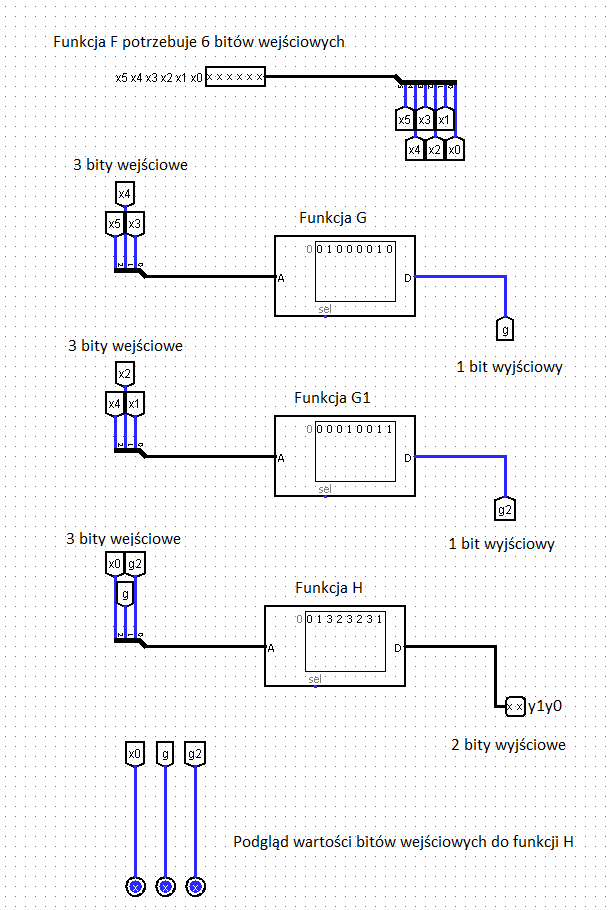
\includegraphics[width=0.95\textwidth]{logisim_all_3.png}
\end{figure}
Zawartość pamięci ROM dla funkcji G
\begin{figure}[H]
	\centering
	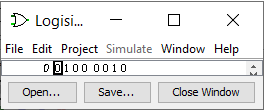
\includegraphics[width=0.5\textwidth]{romG.png}
\end{figure}
Zawartość pamięci ROM dla funkcji G1
\begin{figure}[H]
	\centering
	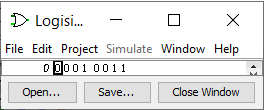
\includegraphics[width=0.5\textwidth]{romG1.png}
\end{figure}
Zawartość pamięci ROM dla funkcji H
\begin{figure}[H]
	\centering
	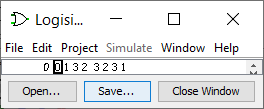
\includegraphics[width=0.5\textwidth]{romH.png}
\end{figure}
\newpage
\begin{center}
    TESTY
\end{center}
5x4x3x2x1=100100
\begin{figure}[H]
	\centering
	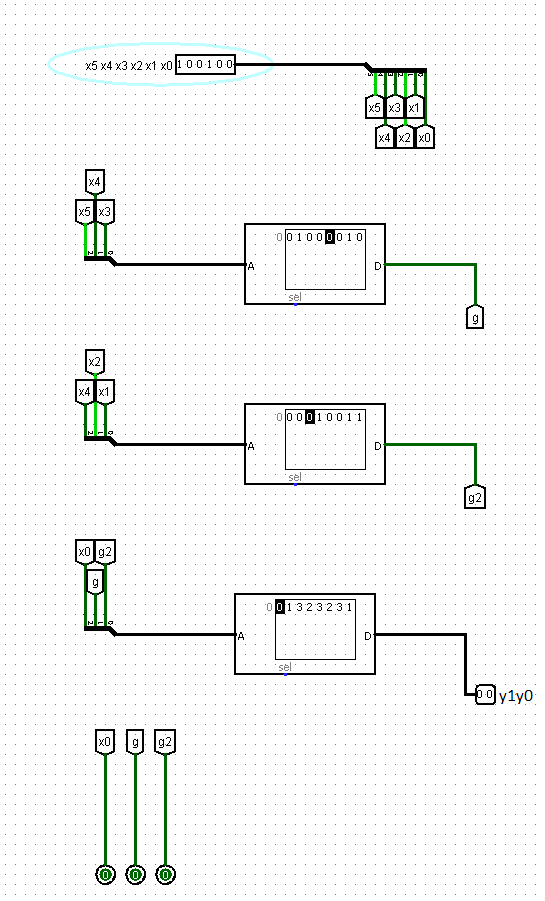
\includegraphics[width=0.88\textwidth]{test3_100100.png}
\end{figure}
x5x4x3x2x1=101110
\begin{figure}[H]
	\centering
	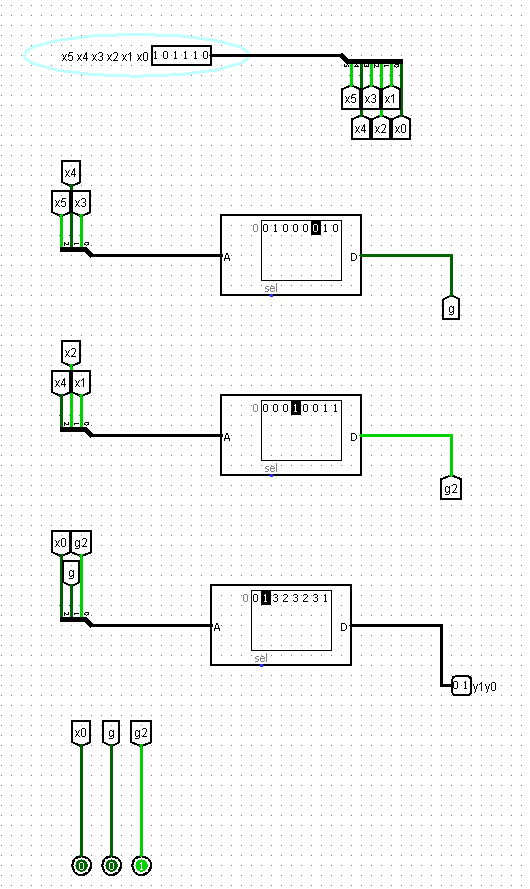
\includegraphics[width=0.88\textwidth]{test3_101110.png}
\end{figure}
x5x4x3x2x1=110111
\begin{figure}[H]
	\centering
	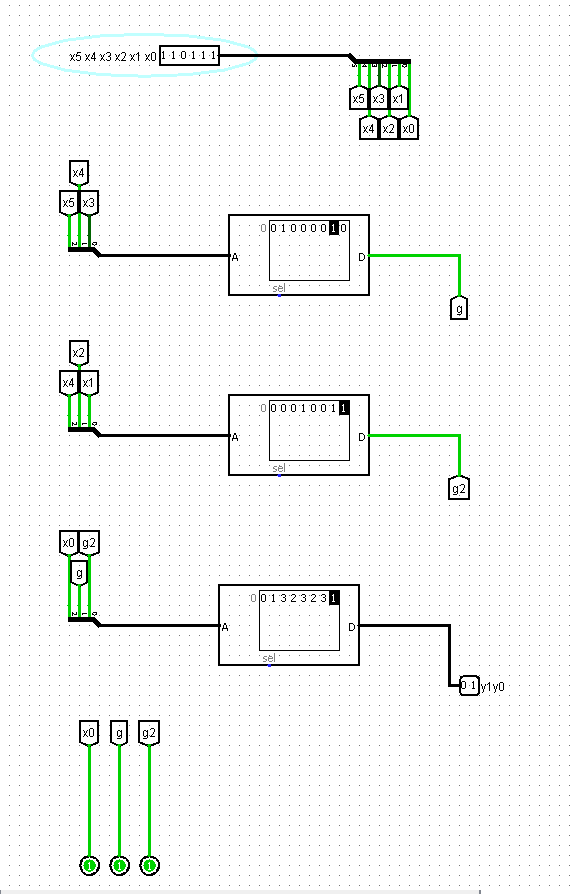
\includegraphics[width=0.88\textwidth]{test3_110111.png}
\end{figure}
\newpage
x5x4x3x2x1=101100
\begin{figure}[H]
	\centering
	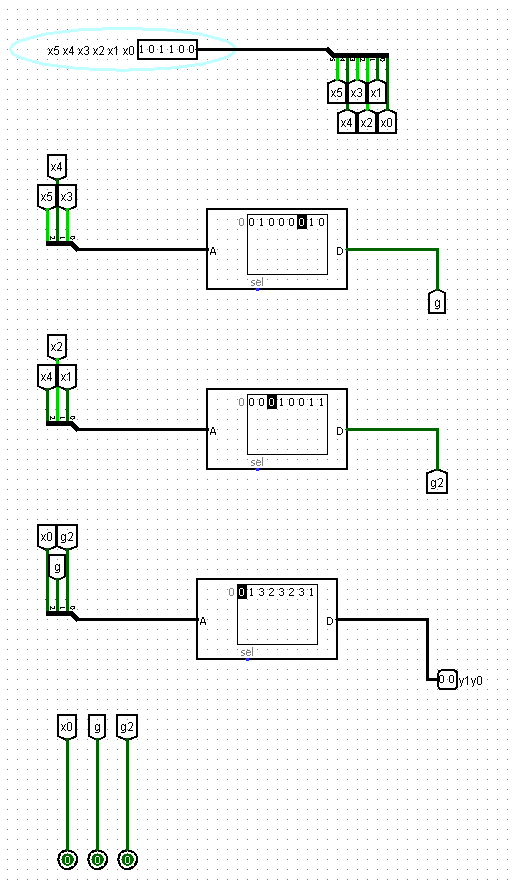
\includegraphics[width=0.88\textwidth]{test3_101100.png}
\end{figure}
x5x4x3x2x1=001110
\begin{figure}[H]
	\centering
	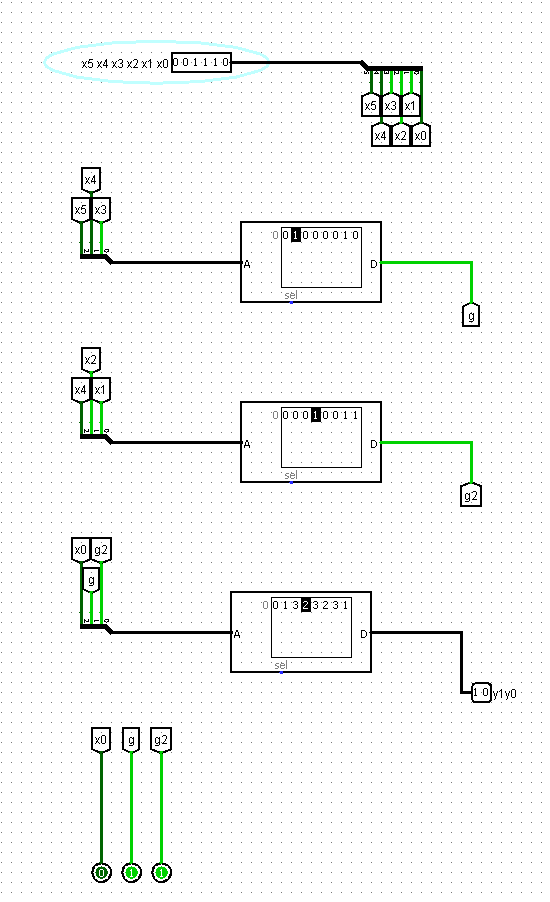
\includegraphics[width=0.88\textwidth]{test3_001110.png}
\end{figure}
\newpage
x5x4x3x2x1=110100
\begin{figure}[H]
	\centering
	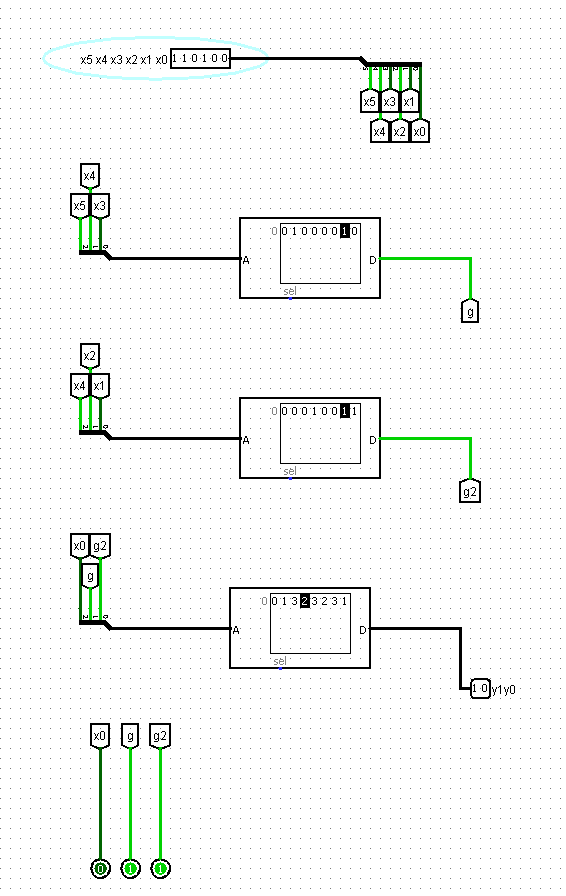
\includegraphics[width=0.88\textwidth]{test3_110100.png}
\end{figure}
\newpage
x5x4x3x2x1=100111
\begin{figure}[H]
	\centering
	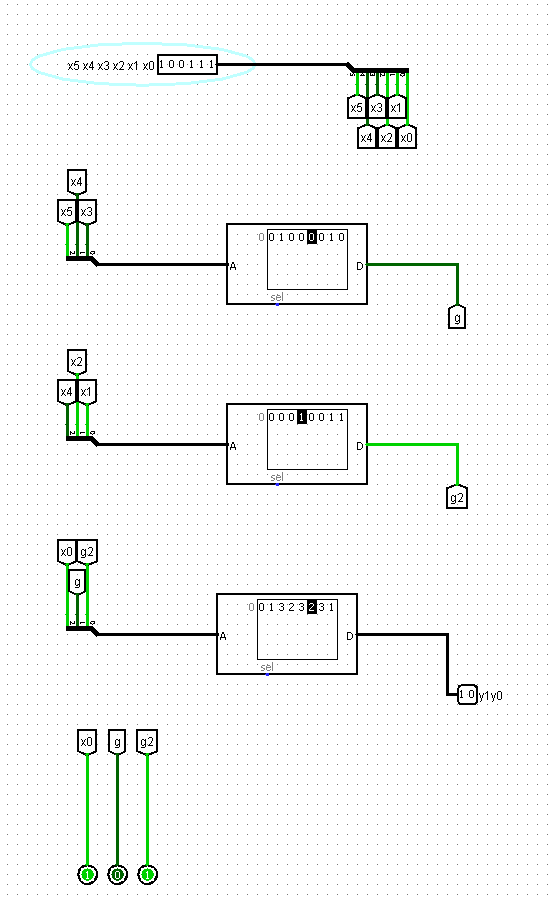
\includegraphics[width=0.88\textwidth]{test3_100111.png}
\end{figure}
\newpage
x5x4x3x2x1=001011
\begin{figure}[H]
	\centering
	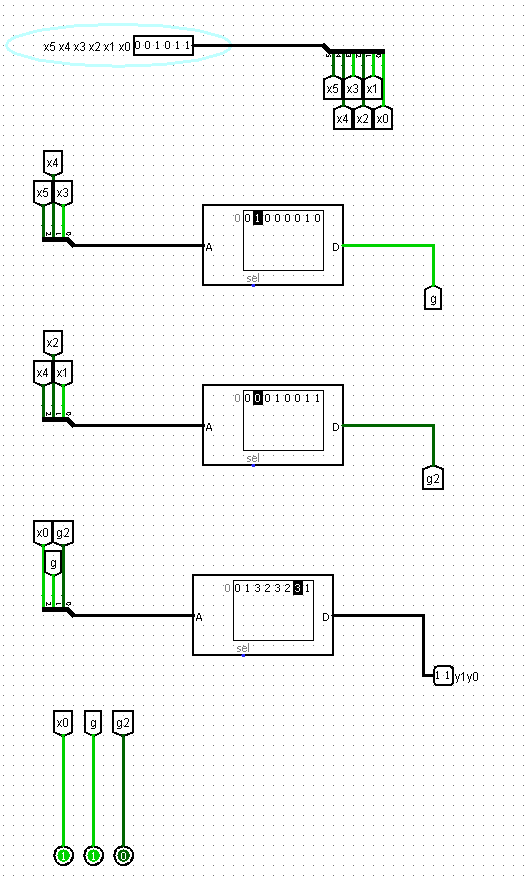
\includegraphics[width=0.88\textwidth]{test3_001011.png}
\end{figure}


\subsection{Realizacja w Quartus}
Tworzymy plik Verilog HDL File o nazwie funkcja\_F. Zakodujemy funkcję F. 
\newline
Zawartość pliku funkcja\_f1:
\begin{lstlisting}[style={prettyverilog}]
module funkcja_F
(   
    input x5,x4,x3,x2,x1,x0,
	 output y1,y0
);	 
wire g,g2;
 
funkcja_G b0 (.x5(x5),.x4(x4),.x3(x3),.g(g));
funkcja_G1 b1 (.x4(x4),.x2(x2),.x1(x1),.g2(g2));
funkcja_H b2 (.x0(x0),.g(g),.g2(g2),.y1(y1),.y0(y0));
 
endmodule
\end{lstlisting}








Tworzymy nowy plik Verilog HDL File o nazwie funkcja\_G. Zakodujemy funkcję G
\newline
Zawartość pliku funkcja\_G:
\begin{lstlisting}[style={prettyverilog}]
module funkcja_G
(
    input x5, x4, x3,
	 output g

);
reg temp;

always@* 
	case ({x5,x4,x3}) 
		3'd4 : temp = 1'd0;
		3'd5 : temp = 1'd0;
		3'd6 : temp = 1'd1;
		3'd1 : temp = 1'd1;
	   default: temp = 1'd0;
    endcase
assign {g} = temp;	 
endmodule
\end{lstlisting}







Tworzymy nowy plik Verilog HDL File o nazwie funkcja\_G1. Zakodujemy funkcję G1.
\newline
Zawartość pliku funkcja\_G1:
\begin{lstlisting}[style={prettyverilog}]
module funkcja_G1
(
    input x4, x2, x1,
	 output g2

);
reg temp;

always@* 
	case ({x4,x2,x1}) 
		3'd1 : temp = 1'd0;
		3'd2 : temp = 1'd0;
		3'd3 : temp = 1'd1;
		3'd6 : temp = 1'd1;
		3'd7 : temp = 1'd1;
	   default: temp = 1'd0;
    endcase
assign {g2} = temp;	 
endmodule
\end{lstlisting}





Tworzymy nowy plik Verilog HDL File o nazwie funkcja\_H. Zakodujemy funkcję H.
\newline
Zawartość pliku funkcja\_H:
\begin{lstlisting}[style={prettyverilog}]
module funkcja_H
(
    input x0, g, g2,
	 output y1,y0

);
reg [0:1] temp;
always@* 
	case ({x0, g, g2}) 
		3'd0 : temp = 2'd0;
		3'd1 : temp = 2'd1;
		3'd2 : temp = 2'd3;
		3'd3 : temp = 2'd2;
		
		3'd4 : temp = 2'd3;
		3'd5 : temp = 2'd2;
		3'd6 : temp = 2'd3;
		3'd7 : temp = 2'd1;
	    default: temp = 2'd0;
    endcase
assign {y1,y0} = temp;	 
endmodule

\end{lstlisting}


\begin{center}
STRUKTURA
\end{center}
\begin{figure}[H]
	\centering
	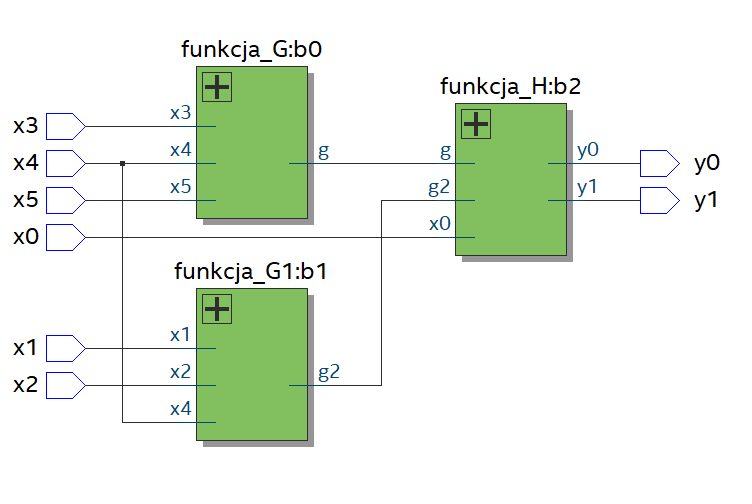
\includegraphics[width=0.70\textwidth]{struktura3.png}
\end{figure}
\newpage
\begin{center}
    Compilation Report
\end{center}

\begin{figure}[H]
	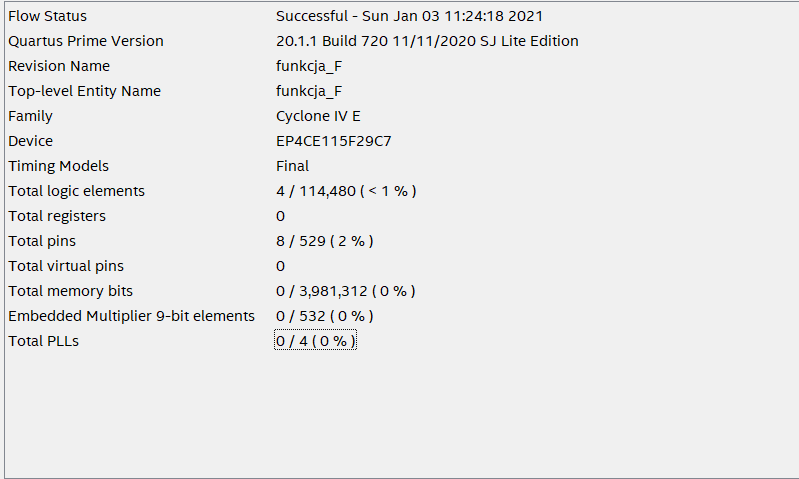
\includegraphics[width=1.2\textwidth]{kompilacja_report3.png}
\end{figure}
\newpage
\subsection{Weryfikacja w ModelSim}
\par Przeprowadzamy symulację w ModelSim.
\begin{figure}[H]
	\centering
	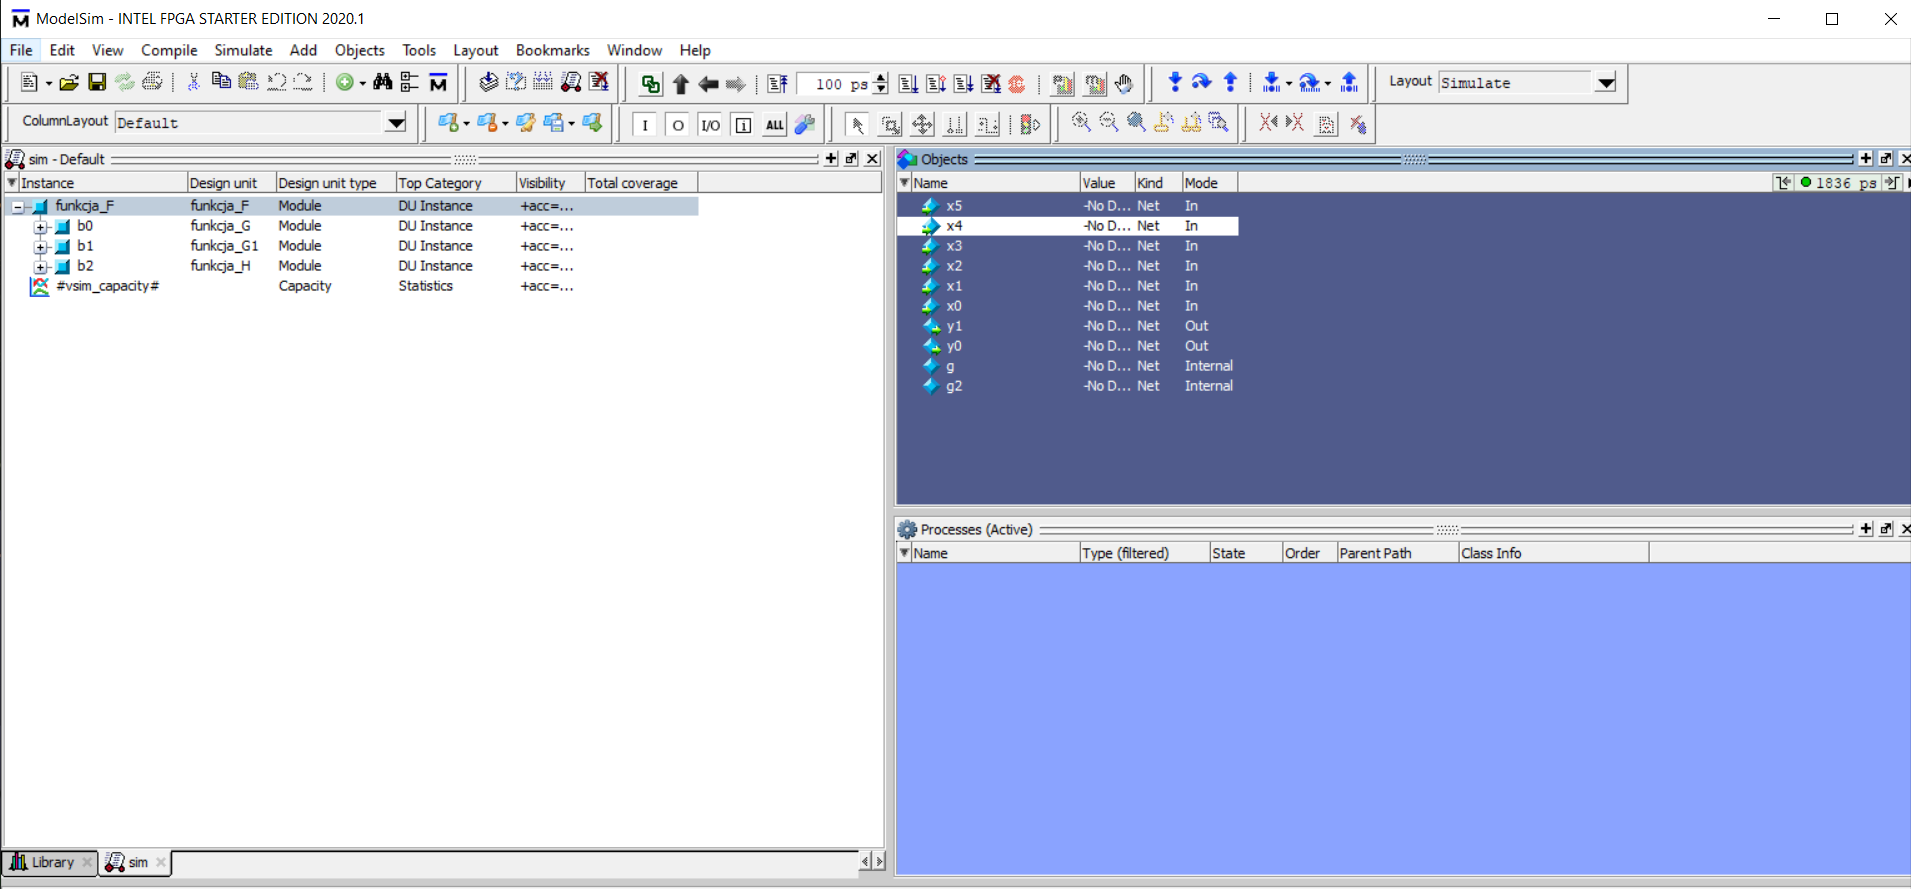
\includegraphics[width=1.25\textwidth]{modelsim3.png}
	\caption{Widok okna ModelSim}
\end{figure}
Sprawdzamy poprawność wyników dla wejść podanych w tabeli prawdy funkcji F. 
\newpage
Zawartość pliku testującego test\_f.do:

\begin{minipage}{0.5\textwidth}
\begin{figure}[H]
	\centering
	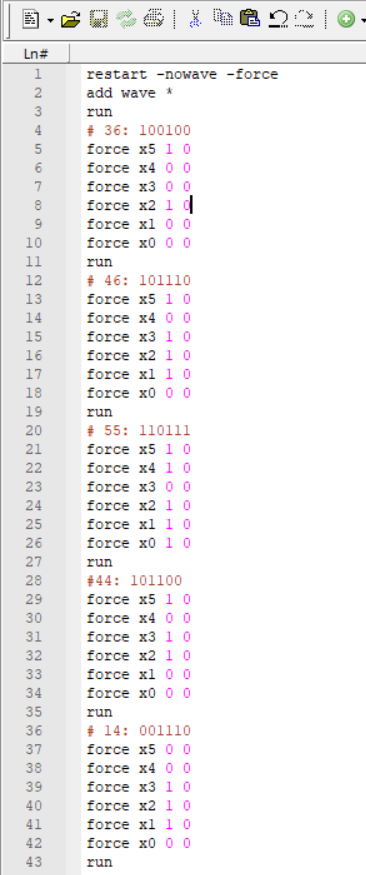
\includegraphics[width=1\textwidth]{test_f3_1.png}
\end{figure}
\end{minipage}
\begin{minipage}{0.5\textwidth}
\begin{figure}[H]
	\centering
	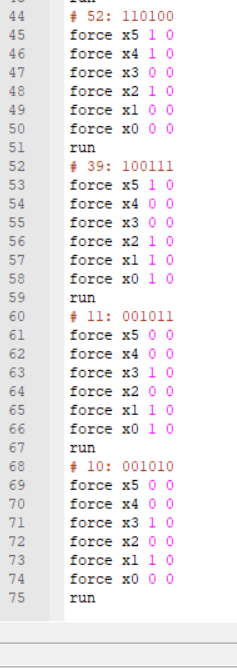
\includegraphics[width=1\textwidth]{test_f3_2.png}
\end{figure}
\end{minipage}
\newpage
\par Widok okna Wave po wykonaniu przez ModelSim polecenia $>$do test\_f.do:
\begin{figure}[H]
	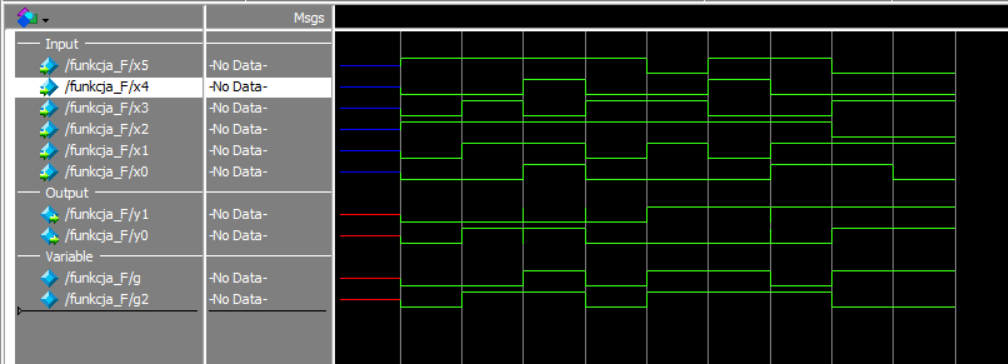
\includegraphics[width=1.25\textwidth]{wave3.png}
\end{figure}
Na podstawie otrzymanych sygnałów zapiszemy tabelę:
\\
\\
\begin{tabular}[]{|c c c c c c |c c|}
\hline
$x_5$ & $x_4$ & $x_3$ & $x_2$ & $x_1$ & $x_0$ & $y_1$ & $y_0$ \\\hline
1 & 0 & 0 & 1 & 0 & 0 & 0 & 0\\
1 & 0 & 1 & 1 & 1 & 0 & 0 & 1\\
1 & 1 & 0 & 1 & 1 & 1 & 0 & 1\\
1 & 0 & 1 & 1 & 0 & 0 & 0 & 0\\
0 & 0 & 1 & 1 & 0 & 0 & 1 & 0\\
1 & 1 & 0 & 1 & 0 & 0 & 1 & 0\\
1 & 0 & 0 & 1 & 1 & 1 & 1 & 0\\
0 & 0 & 1 & 0 & 1 & 1 & 1 & 1\\
0 & 0 & 1 & 0 & 1 & 0 & 1 & 1\\ \hline
\end{tabular}
\\
\\ \textbf{Powstała tabela zgadza się z podaną w treści zadania tabelą funkcji F.}
\end{document}